\documentclass[aspectratio=169,svgnames]{beamer}
\usepackage[utf8]{inputenc}
\usepackage[english]{babel}
\usepackage{mathspec}
\usepackage{minted}
\usepackage{pgfpages}
\usepackage{tikz}
\usepackage{datetime}
\usepackage{xparse}
\usepackage{epigraph}
% \usepackage{enumitem}
\usepackage{fontawesome}
\usepackage{hyperref}
\usepackage[sorting=none]{biblatex}
\usepackage{csquotes}
\usepackage[type={CC}, modifier={by}, version={4.0}]{doclicense}

\newif\ifconcurso
% \concursotrue
\concursofalse

\title[Trabajo de Fin de Grado]{Implementación de una red en chip en un procesador RISC-V}
\subtitle{NoC implementation of a RISC-V processor}
\author[David Davó Laviña]{David~Davó~Laviña\ifconcurso\else\\[1ex] {\scriptsize Óscar Garnica Alcázar \and Juan Lanchares Dávila}\fi}
\institute[UCM]{\ifconcurso\else DACYA, \fi Facultad de Informática, Universidad Complutense de Madrid}
% \date{\today{}}
\date{9 de Junio de 2022}

\useoutertheme{infolines}
\usetheme[height=1.2cm]{Rochester}
\usecolortheme{default}
\setbeamertemplate{navigation symbols}[only frame symbol]{}

\logo{
\includegraphics[height=1cm]{Images/logos/3-2016-07-21-EscudoUCMTransparenteBig.png}}
\titlegraphic{
    
\includegraphics[height=2cm]{Images/logos/3-2016-07-21-EscudoUCMTransparenteBig.png}
    \hspace{.3cm}
    
\includegraphics[height=2cm]{Images/logos/escudofdigrande.png}
    % \hspace{.3cm}
    % \tikz\node[circle, minimum width=1.9cm,
    %     path picture = {
    %         \node at (path picture bounding box.center) {
    %             \includegraphics[width=2cm]{Images/logos/ascii.jpg}
    %         };
    %     }
    % ] {};
}

% Cosas bibliografia
\addbibresource{references.bib}
\setbeamertemplate{bibliography item}{\faFileTextO}
\renewcommand*{\bibfont}{\small}

\begin{document}

\frame[plain]{\titlepage}

\setcounter{tocdepth}{2}
% \begin{frame}[allowframebreaks]{Índice}
\begin{frame}{Índice}
  \tableofcontents
\end{frame}

\section{Introducción y motivaciones}

\begin{frame}{Introducción}
    \setbeamercovered{transparent}
    \begin{block}{Single Event Effects}
        Error en un circuito provocado por una partícula ionizante. (aeroespacial, medicina/ciencia cerca de f. radiación, militar...)
        \pause
        \begin{description}[<+->]
            \item [Soft errors:] Recuperables tras reiniciar el circuito (se resetean los valores iniciales de las señales y se descargan condensadores).
            \item [Hard errors:] Dañan permanentemente parte del circuito.
        \end{description}
    \end{block}
    
    \onslide<+->
    \begin{alertblock}{Solución}
        Reconfiguración Parcial Dinámica en FPGAs + \textbf{Redes de Interconexión}
    \end{alertblock}
    
    \nocite{BinderAnomalies}
\end{frame}

\ifconcurso
    % No menciono los objetivos
\else
    \section{Objectives}
    
    \begin{frame}{Objectives}
        \begin{itemize}
            \item Choose a RISC-V implementation to study and modify
            \item Specify the features of the NoC, describe it using HDL and simulate.
            \item Integrate the NoC inside RISC-V RTL, simulate resulting design
            \item Make sure the created designs are synthetizable
        \end{itemize}
    \end{frame}
\fi
\section{RISC-V}

\begin{frame}{RISC-V}
    \begin{itemize}
        \item Libre y gratuita
        \item Conjunto de instrucciones reducido (RISC)
        \item Registro a Registro o load/store
        \item Modular
    \end{itemize}
    
    \nocite{RiscVSpec1}
    \nocite{RiscVExchangeCores}
\end{frame}

\begin{frame}{Familia SweRV}
    \begin{figure}
        \centering
        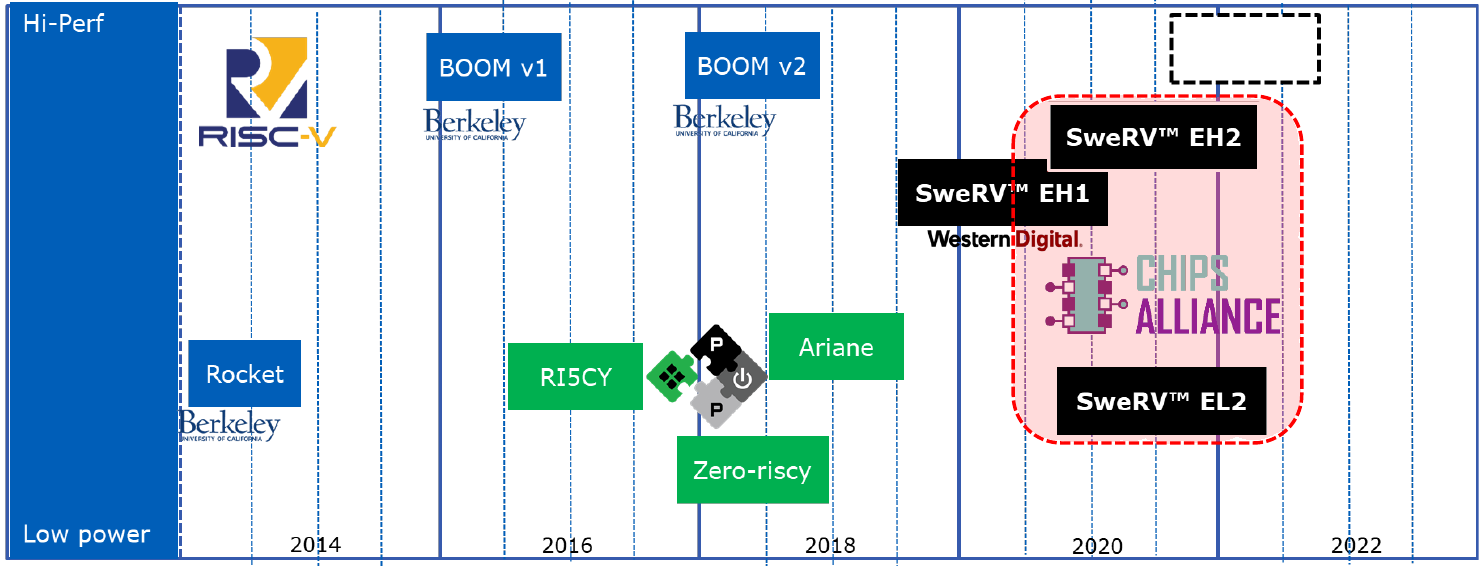
\includegraphics[width=.7\linewidth]{Images/roadmap_compare2.png}
        \caption{Comparativa de la potencia de varios Cores RISC-V de código abierto. Extraído de \citetitle{SweRVRoadmap}~\cite{SweRVRoadmap}.}
        \label{fig:roadmap_compare}
    \end{figure}
    
    \nocite{RepoSwervEL2}
\end{frame}

\begin{frame}{Microarquitectura SweRV-EL2}
        \begin{columns}[t]
            \column{.5\linewidth}
            \begin{figure}[t]
                \centering
                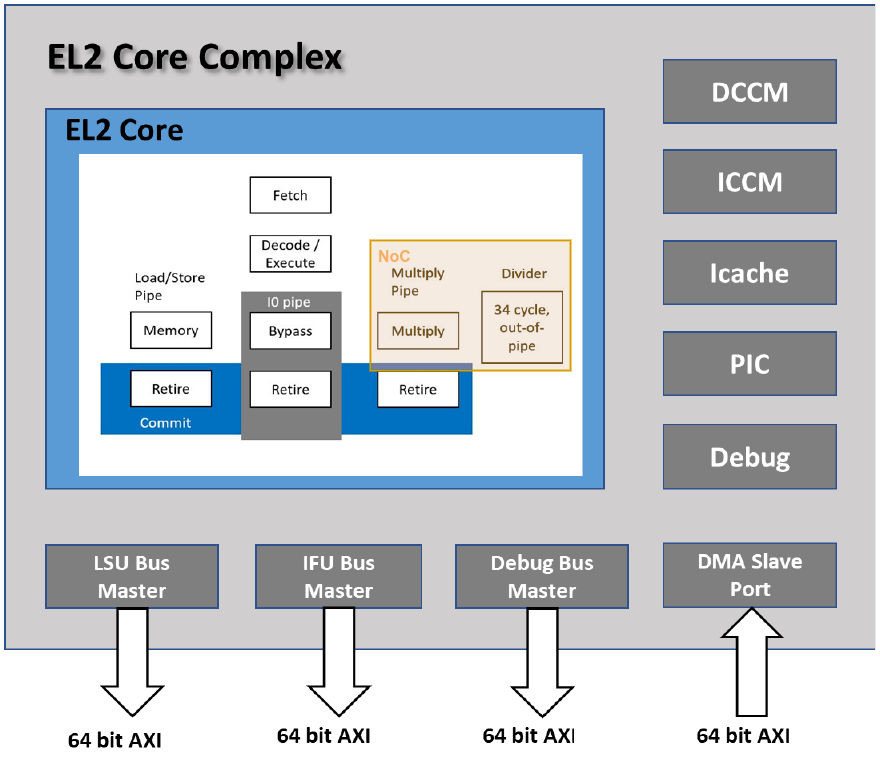
\includegraphics[width=.70\linewidth]{Images/swerv_architecture.drawio2.png}
                \caption{Complejo del SweRV-EL2. Señalado en naranja las partes que hacen uso de la NoC. Extraído de \citetitle{SweRVRoadmap}~\cite{SweRVRoadmap}.}
                \label{fig:swerv_complex}
            \end{figure}%
            \column{.5\linewidth}\pause%
            \begin{figure}[t]
                \centering
                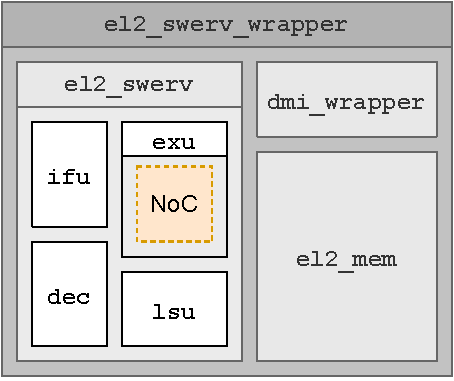
\includegraphics[width=.75\linewidth]{Images/swerv_blocks.drawio.pdf}
                \caption{Diagrama de bloques del procesador modificado.}
                \label{fig:swerv_blocks}
            \end{figure}
        \end{columns}
\end{frame}

\section{Network on Chip}

\nocite{HenessyPattersonCAQA}
\nocite{AC5}
\nocite{HenessyPattersonF}
\nocite{Duato03}
\nocite{YalamanchiliPCS}
\nocite{DeMicheli2006NetworksTools}

\subsection{Características de la red}
\begin{frame}{Características de la red I}
    \begin{minipage}[t]{.5\textwidth}
        \begin{figure}
            \centering
            \caption{Topología en malla indirecta}
            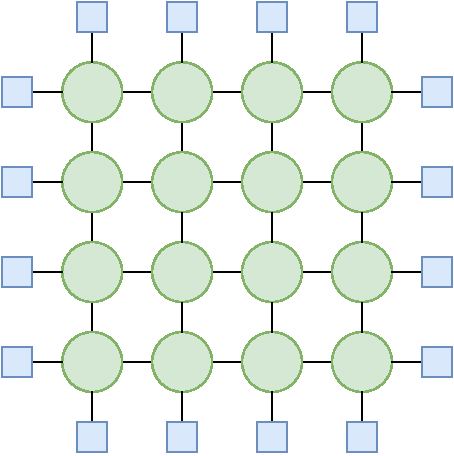
\includegraphics[width=.6\linewidth]{Images/topology_mesh_edge.drawio.pdf}
            \label{fig:topology}
        \end{figure}
    \end{minipage}\pause\begin{minipage}[t]{.5\textwidth}
        \begin{figure}
            \centering
            \caption{Encaminamiento en Orden Dimensional}
            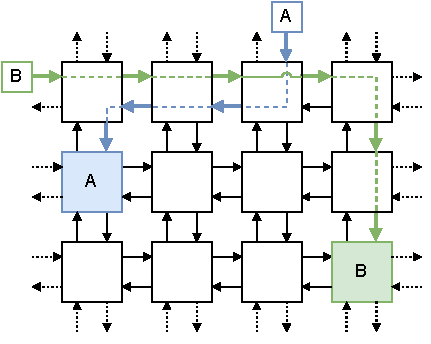
\includegraphics[width=.8\linewidth]{Images/dor2.drawio.pdf}
            \label{fig:routing}
        \end{figure}
    \end{minipage}
\end{frame}

\begin{frame}{Características de la red II}
    \begin{figure}
        \centering
        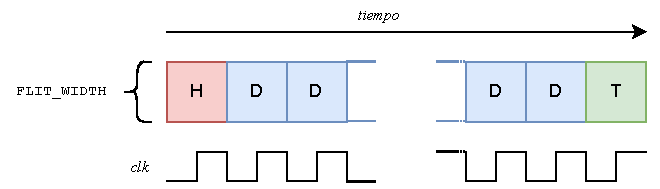
\includegraphics[width=.7\linewidth]{Images/packets.drawio.pdf}
        \caption{Envío de varios flits para formar un paquete.}
        \label{fig:packet}
    \end{figure}
\end{frame}

\subsection{Integración en el SweRV-EL2}

\begin{frame}{Modulos creados}
    \setbeamercovered{transparent}
    \begin{block}{Módulos de Red}
        \begin{itemize}[<+->]
            \item \textbf{Malla}: Instancia una malla bidimensional de \textit{router}s.
            \item \textbf{Router}: Hace de encaminador y tiene un \textit{crossbar}.
            \item \textbf{Crossbar}: Realiza la conmutación
        \end{itemize}
    \end{block}
    \onslide<+->
    \begin{block}{Módulos de Integración}
        \begin{itemize}[<+->]
            \item \textbf{Emisor}: Recibe un dato de longitud fija por un bus, lo empaqueta, y lo envía en una serie de flits por la red.
            \item \textbf{Receptor}: Recibe flits de la red, los desempaqueta en registros, y provee los resultados en un bus.
            \item \textbf{Wrapper}: Instancia un \textit{receptor}, el elemento de la EXU, y un \textit{emisor}.
        \end{itemize}
    \end{block}
\end{frame}

\begin{frame}{Integración de la NoC en el SweRV-EL2}
    \centering
    \only<1>{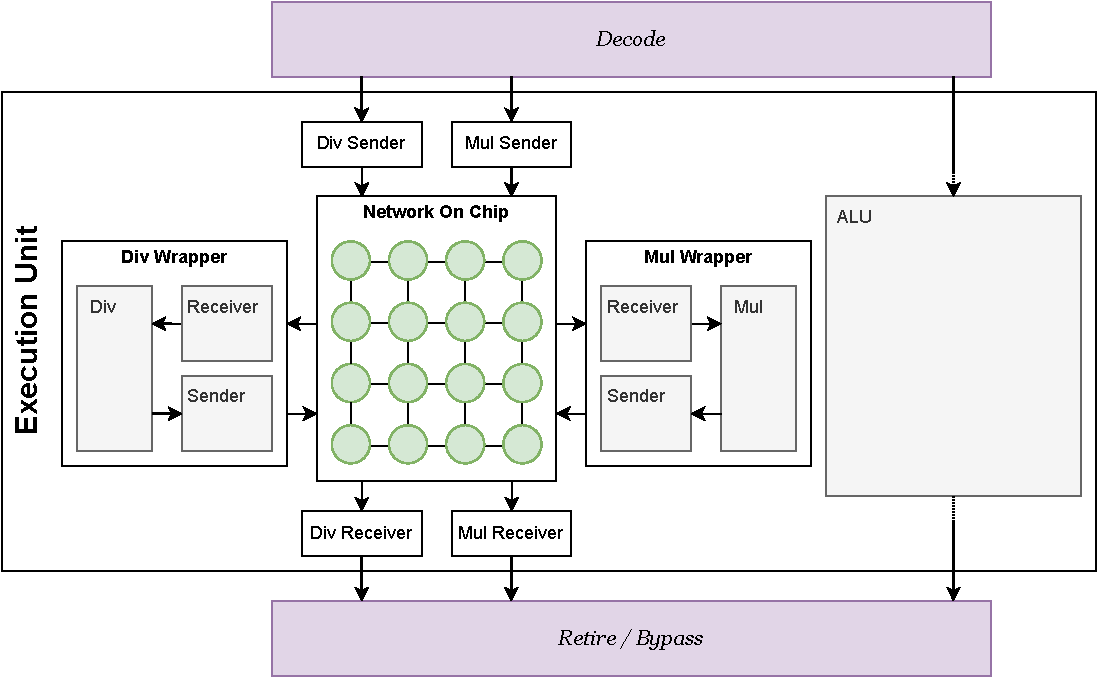
\includegraphics[height=.9\textheight]{Images/sketch_wrappers_horizontal.drawio.pdf}}
    \only<2>{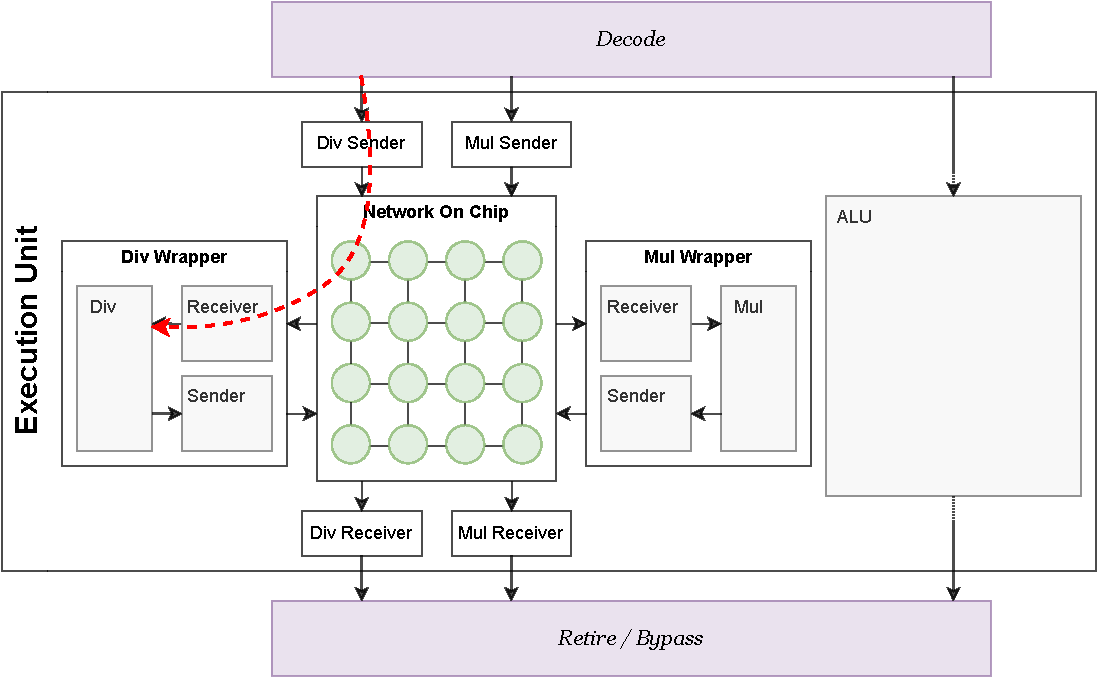
\includegraphics[height=.9\textheight]{Images/sketch_wrappers_horizontal-Page-3.drawio.pdf}}
    \only<3>{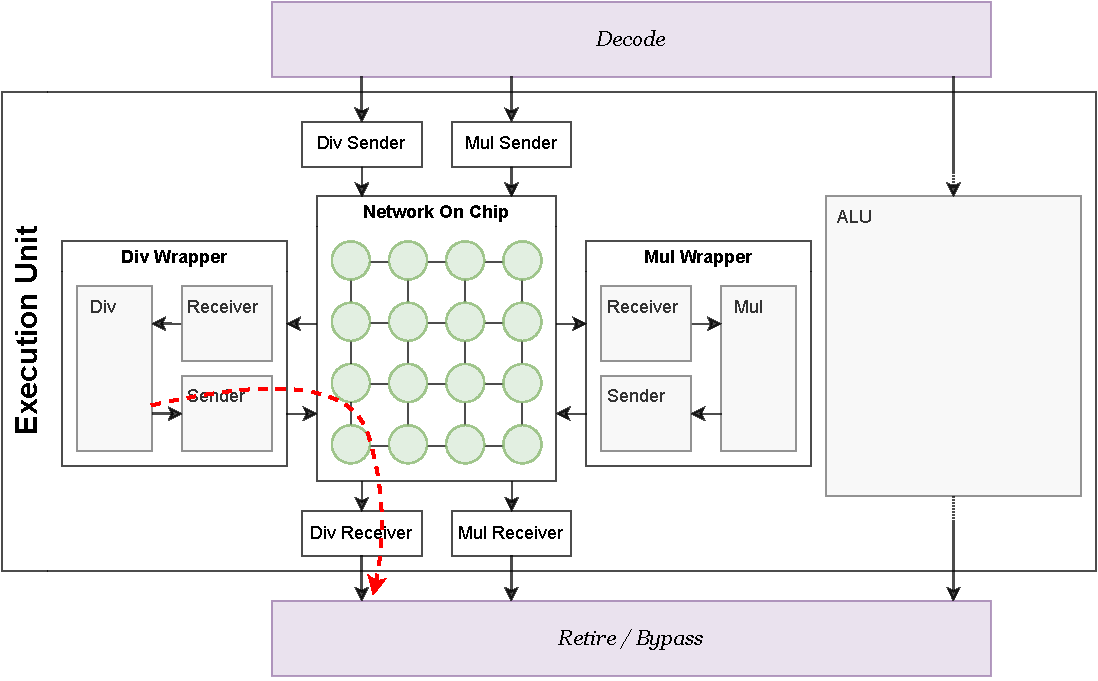
\includegraphics[height=.9\textheight]{Images/sketch_wrappers_horizontal-Page-4.drawio.pdf}}
\end{frame}
\section{Resultados}

\begin{frame}{Resultados de simulación: NoC}
    \begin{minipage}{.5\textwidth}
        \centering
        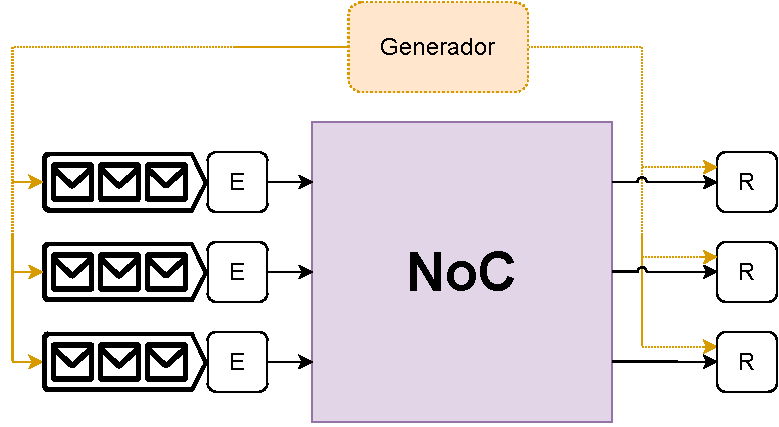
\includegraphics[width=\linewidth]{Images/testbench.drawio.pdf}
    \end{minipage}\pause\begin{minipage}{.5\textwidth}
        \centering
        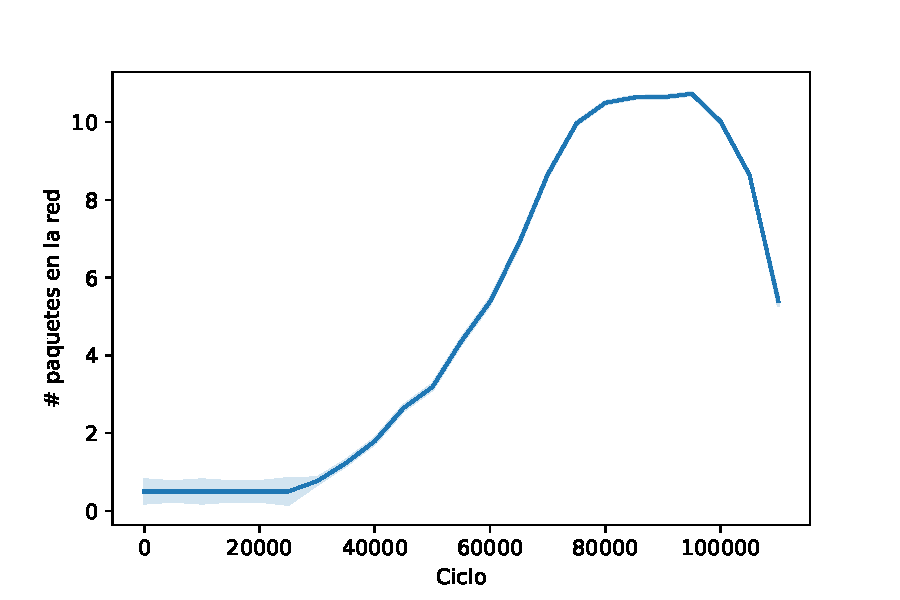
\includegraphics[width=\linewidth]{Images/packets.pdf}
    \end{minipage}
\end{frame}

\begin{frame}{Resultados de simulación: SweRV-EL2}
    \begin{minipage}{.5\textwidth}
        \centering
        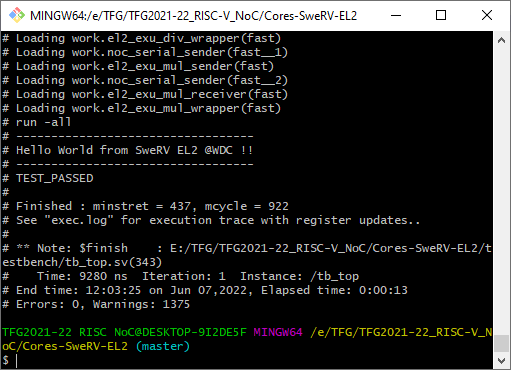
\includegraphics[width=.95\linewidth]{Images/captura_hello_world.PNG}
    \end{minipage}\begin{minipage}{.5\textwidth}
        \centering
        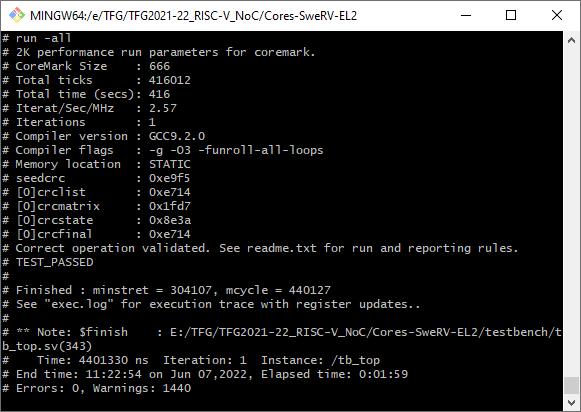
\includegraphics[width=.95\linewidth]{Images/captura_coremark.PNG}
    \end{minipage}
\end{frame}

\begin{frame}{Resultados de síntesis}
    \centering
    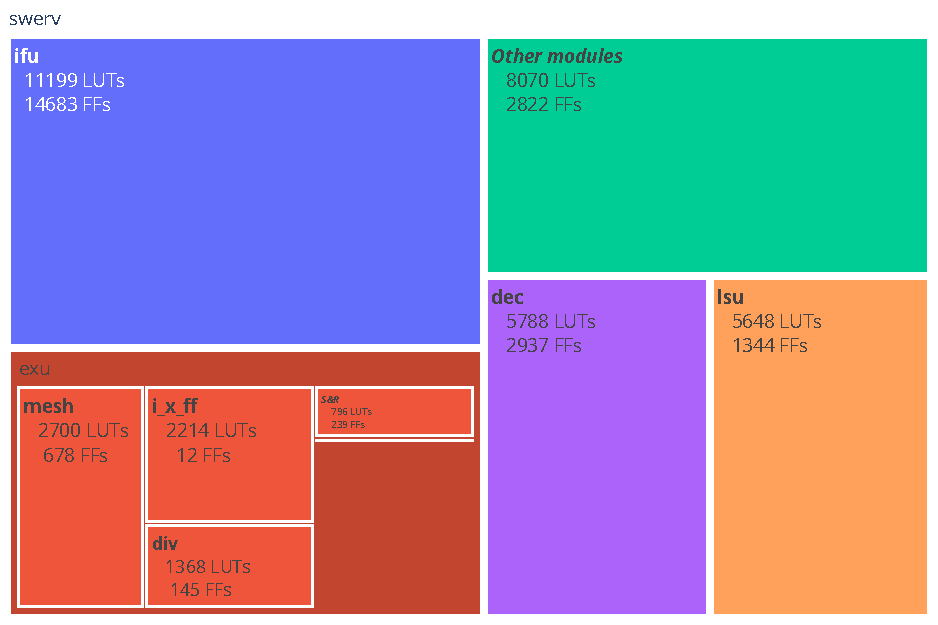
\includegraphics[height=.9\textheight]{Images/swerv_treemap.pdf}
\end{frame}
\section{Trabajo futuro y conclusiones}

\begin{frame}{Trabajo futuro}
    \begin{itemize}
        \item Monitorización de la red
        \item Optimización de recursos consumidos
        \item Comprobación de errores
        \item Encaminamiento adaptativo
        \item Continuar con el flujo de diseño $\rightarrow$ Implementación en FPGA y prueba
    \end{itemize}
\end{frame}

\begin{frame}{Conclusiones}
    \begin{itemize}
        \item Diseño RTL sintetizable de una NoC
        \item Modificado el diseño del SweRV-EL2 incluyendo una NoC
        \item Aprendizaje de SystemVerilog, testbenches automatizados, síntesis con Xilinx Vivado y simulación y depuración en QuestaSim
    \end{itemize}
\end{frame}

\section{Referencias}
\begin{frame}[allowframebreaks]{Referencias}
    % \nocite{*}
    % \bibliographystyle{plain}
    % \bibliographystyle{acm}
    \printbibliography
\end{frame}

\end{document}
